\chapter{Microcontroladores: História e Arquitetura}
\label{cap:arquitetura-mcu}

Antes de configurar o ambiente de desenvolvimento e escrever firmware de verdade, vale entender de onde vêm os microcontroladores e como sua unidade de processamento funciona por dentro. Esse pano de fundo explica \emph{por que} o firmware que escreveremos ao longo desta apostila é estruturado do jeito que é — e, em particular, por que o \ESP{} precisa ser protegido por um mecanismo chamado \textbf{Watchdog Timer}, apresentado ao final deste capítulo.

\section{Um breve histórico}

Desenvolver um novo circuito eletrônico dedicado a cada novo projeto consome muito tempo e recursos. Cada nova função exigiria, literalmente, um novo circuito projetado do zero. Foi para resolver esse problema que o engenheiro \textbf{Federico Faggin}, então na Intel, ajudou a desenvolver um circuito capaz de executar um \textbf{conjunto de operações em uma sequência definida}, armazenada em uma memória — em vez de um circuito fixo, um circuito \emph{programável}. Essa mudança de perspectiva é o que separa um circuito puramente digital (como os circuitos combinacionais e sequenciais estudados em eletrônica digital) de um \textbf{processador}: em vez de redefinir o hardware para cada nova tarefa, basta escrever uma nova sequência de instruções.

O primeiro produto comercial desse tipo foi o chip \textbf{Intel 4004}, desenvolvido para equipar a calculadora \emph{Busicom 141-PF}.

\begin{figure}[h]
\centering
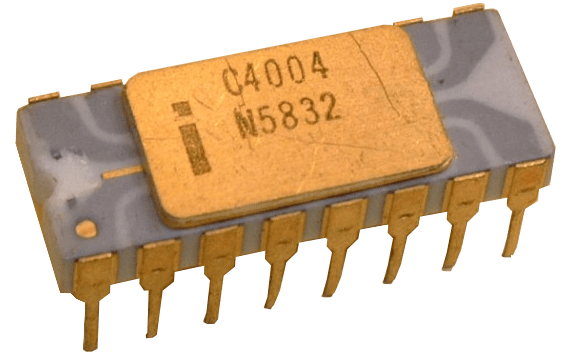
\includegraphics[width=0.45\textwidth]{imagens/intel_4004.png}
\caption{O Intel 4004 (1971), o primeiro microprocessador comercial.}
\end{figure}

Lançado em 1971, o Intel 4004 possuía uma arquitetura de apenas \textbf{4 bits}, um repertório de \textbf{45 instruções} diferentes, e operava a uma frequência de \emph{clock} máxima de \textbf{740 kHz} — para comparação, milhares de vezes mais lento que o \ESP{} que usaremos nesta apostila.

Um microprocessador sozinho, porém, não é suficiente para compor um circuito integrado completo para aplicações embarcadas: ele ainda precisaria de chips externos de memória e de interface para ser útil. Foi para resolver essa lacuna que surgiram os \textbf{microcontroladores} — circuitos integrados que reúnem, em um único chip:

\begin{itemize}
    \item a \textbf{ROM} (\emph{Read-Only Memory}), associada às instruções do programa;
    \item a \textbf{RAM} (\emph{Random-Access Memory}), associada aos dados manipulados durante a execução;
    \item registradores digitais de \textbf{interface} com dispositivos externos — os pinos GPIO e periféricos apresentados no \cref{cap:embarcados}.
\end{itemize}

Esse é, essencialmente, o mesmo modelo — bastante amadurecido e miniaturizado — que encontramos hoje dentro do \ESP{}.

\section{A unidade de processamento}

A \textbf{unidade de processamento} (ou simplesmente \emph{processador}) é o centro de um microcontrolador: é ela quem coordena, executa e gerencia todos os recursos disponíveis. Do ponto de vista da eletrônica digital, essa unidade é um \textbf{circuito sequencial} — ou seja, seu \textbf{estado atual} combinado aos \textbf{dados de entrada} determina qual será o \textbf{próximo estado} que o circuito assumirá.

Essas transições de estado acontecem de forma \textbf{síncrona}, ritmadas por um sinal elétrico periódico chamado \textbf{\emph{clock}}. O intervalo de tempo entre duas transições consecutivas é chamado de \textbf{ciclo}.

\begin{figure}[h]
\centering
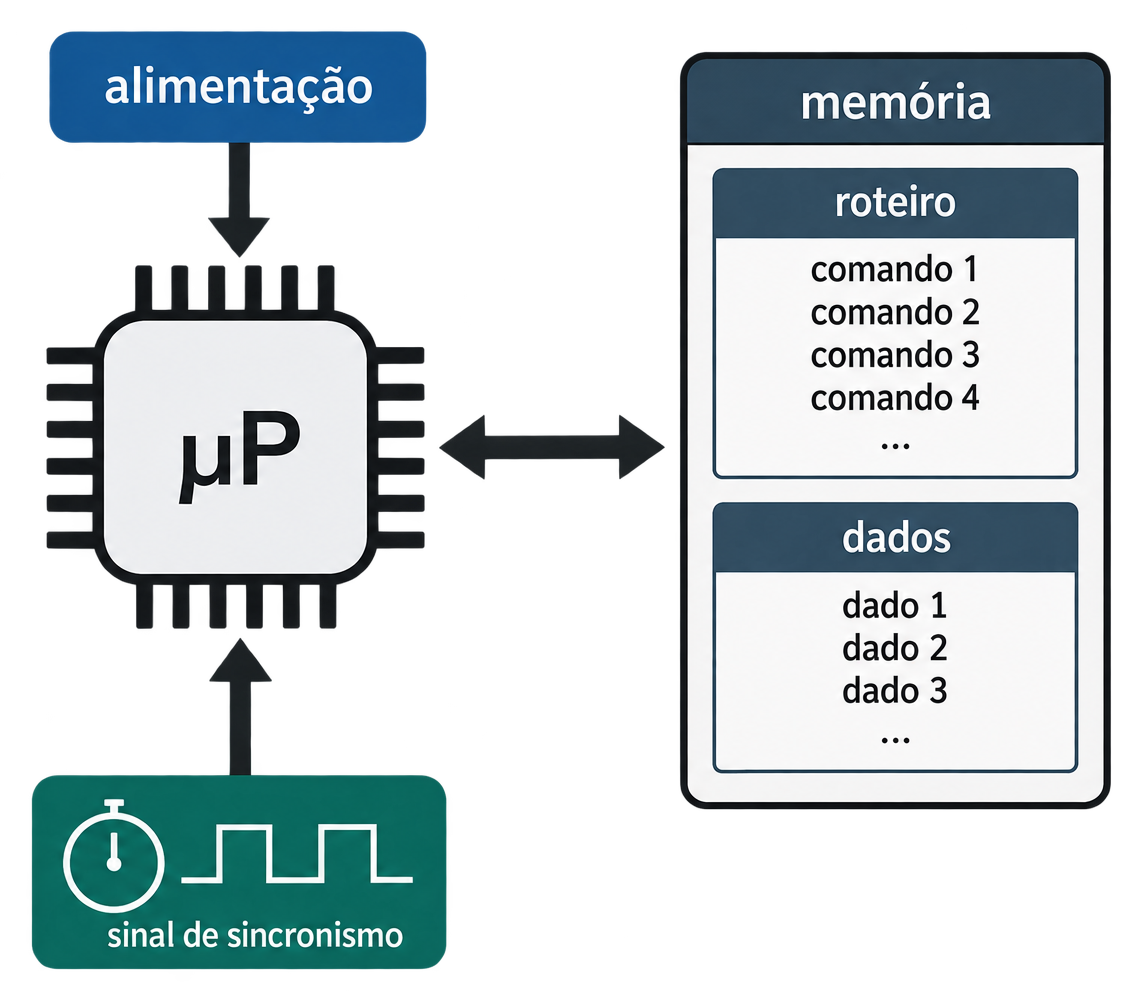
\includegraphics[width=0.72\textwidth]{imagens/estado_microcontrolador.png}
\caption{Visão simplificada de uma unidade de processamento ($\mu$P): alimentação, sinal de sincronismo (\emph{clock}) e o barramento bidirecional de acesso à memória, contendo o roteiro de instruções e os dados do programa.}
\end{figure}

Em cada ciclo, o processador busca a próxima instrução do \textbf{roteiro} (o programa, armazenado na memória de instruções), interpreta o que ela pede para fazer, e a executa — lendo ou escrevendo \textbf{dados}, atualizando registradores, ou desviando para outra instrução. É exatamente essa sequência de busca-decodificação-execução, repetida indefinidamente a cada ciclo de \emph{clock}, que dá vida ao código C que escrevemos: cada linha do seu programa, depois de compilada, se transforma em uma ou mais dessas instruções elementares.

\begin{nota}
Um aprofundamento completo sobre o projeto interno de processadores — unidades de controle, bancos de registradores, pipelines — foge do escopo desta apostila introdutória, mas é um tema fascinante para quem quiser entender ainda melhor o que acontece ``por baixo'' do código C.
\end{nota}

\section{Arquitetura de laço único (\emph{Super Loop})}
\label{sec:super-loop}

Com o hardware entendido em linhas gerais, resta uma pergunta: como \emph{organizar} o firmware que roda sobre ele? A resposta mais simples — e, ainda hoje, a mais usada em projetos de pequeno e médio porte — é a chamada \textbf{arquitetura de laço único} (em inglês, \emph{Super Loop} ou \emph{bare-metal loop}).

A ideia é direta: o firmware é dividido em duas fases.

\begin{enumerate}
    \item Uma fase de \textbf{inicialização}, executada uma única vez, ao ligar o dispositivo — configurar pinos, iniciar periféricos, preparar variáveis;
    \item Um \textbf{laço infinito}, executado indefinidamente depois disso, dentro do qual todas as tarefas do sistema são verificadas e atualizadas repetidamente, uma volta atrás da outra, para sempre.
\end{enumerate}

Você já reconhece essa estrutura: é exatamente o par \code{setup()} / \code{loop()} do framework Arduino, apresentado no \cref{cap:anatomia}. \code{setup()} é a fase de inicialização; \code{loop()}, chamada repetidamente pelo próprio framework, é o laço único.

A grande vantagem da arquitetura de laço único é a \textbf{simplicidade}: não há troca de contexto entre tarefas, não há concorrência para gerenciar, e o comportamento do sistema é fácil de prever e depurar — a cada volta do laço, o código roda sempre na mesma ordem. É também extremamente econômica em termos de memória, o que a torna ideal para microcontroladores simples.

O preço dessa simplicidade é que \textbf{nenhuma tarefa pode bloquear o laço por muito tempo}. Se uma única iteração de \code{loop()} demorar demais — por exemplo, presa em um \code{delay()} longo ou esperando um sensor lento —, \emph{todo} o resto do sistema fica paralisado durante esse tempo: nenhum outro sensor é lido, nenhum outro botão é verificado. É exatamente por isso que o \cref{cap:interrupcoes} apresenta a técnica de temporização por \code{millis()} como alternativa ao \code{delay()} dentro de um laço com múltiplas responsabilidades — e é para proteger o sistema quando, apesar de tudo, alguma tarefa trava por completo, que existe o mecanismo apresentado a seguir.

\section{Watchdog Timer}
\label{sec:watchdog}

Mesmo em um firmware bem projetado, coisas dão errado: um sensor pode parar de responder e travar uma leitura que deveria ser rápida, um laço de espera pode nunca satisfazer sua condição de saída, ou um bug qualquer pode prender a execução em um ponto do código do qual ela nunca retorna. Em uma arquitetura de laço único (\cref{sec:super-loop}), isso é particularmente grave: se \code{loop()} trava, \textbf{o sistema inteiro trava} — sem um sistema operacional completo para intervir, nada tira o processador desse estado sozinho.

A solução para esse problema é um pequeno circuito de hardware chamado \textbf{Watchdog Timer} (WDT, ou ``temporizador de vigilância''): um contador regressivo independente que, se não for \textbf{reiniciado periodicamente pelo próprio firmware}, entende que o sistema travou e força um \textbf{reset} completo do microcontrolador — trazendo-o de volta a um estado conhecido e funcional, em vez de deixá-lo preso indefinidamente.

O uso típico segue um padrão de três passos:

\begin{enumerate}
    \item \textbf{Configurar} o watchdog com um tempo limite (\emph{timeout}) — por exemplo, 5 segundos;
    \item Dentro do laço principal, \textbf{alimentar} (``dar comida a'') o watchdog periodicamente, sempre que o firmware sabe que está funcionando normalmente — isso reinicia a contagem regressiva;
    \item Se, por qualquer motivo, o firmware travar e parar de alimentar o watchdog, o tempo limite se esgota e o \textbf{chip reinicia sozinho}.
\end{enumerate}

\begin{codigoc}{src/main.cpp — protegendo o laço principal com o watchdog}
#include <esp_task_wdt.h>

#define WDT_TIMEOUT 5   // segundos ate o reset, caso nao seja alimentado

void setup() {
    Serial.begin(115200);

    esp_task_wdt_init(WDT_TIMEOUT, true);   // true: reinicia o chip ao vencer
    esp_task_wdt_add(NULL);                 // registra a tarefa de loop() no watchdog

    Serial.println("Watchdog configurado. Sistema iniciado.");
}

void loop() {
    // ... leitura de sensores, logica do programa, etc ...

    Serial.println("Laco em execucao normal.");
    esp_task_wdt_reset();   // "alimenta" o watchdog: avisa que o laco esta vivo

    delay(1000);
}
\end{codigoc}

\begin{dica}
Para ver o watchdog em ação, tente comentar a linha \code{esp\_task\_wdt\_reset();} e substituir o \code{delay(1000)} por um laço vazio bem mais longo que o \code{WDT\_TIMEOUT} configurado (por exemplo, \code{while (true) \{\}}). Poucos segundos depois, o watchdog vai perceber que o laço parou de ser alimentado e reiniciar o \ESP{} sozinho — o monitor serial mostrará a mensagem \code{"Sistema iniciado."} aparecendo repetidamente, uma prova visível de que o mecanismo de proteção está funcionando.
\end{dica}

\begin{atencao}
Chamar \code{esp\_task\_wdt\_reset()} em um ponto do código onde, na verdade, algo já está errado — por exemplo, dentro de um laço de espera que deveria ter um limite de tentativas — \textbf{mascara o problema} em vez de resolvê-lo: o watchdog nunca vai disparar, mesmo que o sistema esteja preso ali, inútil, indefinidamente. O watchdog deve alimentar-se a partir de um ponto do código que só é alcançado quando o laço principal de fato completou uma volta inteira e saudável — nunca de dentro de uma espera que já é, ela própria, suspeita.
\end{atencao}

Com o histórico e a arquitetura de um microcontrolador em mente, o próximo capítulo coloca a mão na massa: a instalação e configuração do \textbf{PlatformIO}, o ambiente que usaremos para escrever, compilar e carregar firmware no \ESP{}.
